\documentclass[12pt,a4paper]{report}
\usepackage[utf8]{inputenc}
\usepackage[russian]{babel}
\usepackage{amsmath}
\usepackage{amsfonts}
\usepackage{amssymb}
\usepackage{graphicx}
\usepackage{geometry}
\usepackage{float}
\usepackage{listings}
\usepackage{xcolor}
\usepackage{hyperref}
\usepackage{titlesec}
\usepackage{fancyhdr}
\usepackage{tocloft}

\geometry{left=2.5cm,right=2.5cm,top=2.5cm,bottom=2.5cm}

% Настройка заголовков
\titleformat{\chapter}[display]
{\normalfont\huge\bfseries}{\chaptertitlename\ \thechapter}{20pt}{\Huge}

% Настройка колонтитулов
\pagestyle{fancy}
\fancyhf{}
\fancyhead[R]{\thepage}
\fancyhead[L]{Лабораторная работа №1}

% Настройка кода
\lstset{
    language=Python,
    basicstyle=\ttfamily\small,
    keywordstyle=\color{blue},
    commentstyle=\color{green!60!black},
    stringstyle=\color{red},
    numbers=left,
    numberstyle=\tiny\color{gray},
    stepnumber=1,
    numbersep=5pt,
    frame=single,
    breaklines=true,
    breakatwhitespace=true,
    tabsize=4
}

% Гиперссылки
\hypersetup{
    colorlinks=true,
    linkcolor=blue,
    filecolor=magenta,      
    urlcolor=cyan,
    pdftitle={Лабораторная работа №1},
    pdfauthor={Студент}
}

\begin{document}

% Титульный лист
\begin{titlepage}
    \centering
    \vspace*{1cm}
    
    {\Large\textbf{МИНИСТЕРСТВО НАУКИ И ВЫСШЕГО ОБРАЗОВАНИЯ РОССИЙСКОЙ ФЕДЕРАЦИИ}}
    
    \vspace{1cm}
    
    {\large\textbf{ФЕДЕРАЛЬНОЕ ГОСУДАРСТВЕННОЕ АВТОНОМНОЕ ОБРАЗОВАТЕЛЬНОЕ УЧРЕЖДЕНИЕ ВЫСШЕГО ОБРАЗОВАНИЯ}}
    
    \vspace{0.5cm}
    
    {\large\textbf{НАЦИОНАЛЬНЫЙ ИССЛЕДОВАТЕЛЬСКИЙ УНИВЕРСИТЕТ ИТМО}}
    
    \vspace{2cm}
    
    {\Large\textbf{Лабораторная работа №1}}
    
    \vspace{0.5cm}
    
    {\Large\textbf{Уменьшение размерности данных и сравнение методов}}
    
    \vspace{1cm}
    
    \begin{flushleft}
    \textbf{Дисциплина:} Современные инструменты анализа данных
    
    \textbf{Тема:} Методы уменьшения размерности: PCA и t-SNE
    
    \vspace{1cm}
    
    \textbf{Выполнил:} Студент группы K3341 Меньшенин Евгений
    
    \end{flushleft}
    
    \vfill
    
    {\large Санкт-Петербург \the\year}
    
\end{titlepage}

% Содержание
\tableofcontents
\newpage

% Введение
\chapter{Введение}

\section{Цель работы}

Освоить практические навыки работы с методами уменьшения размерности данных, такими как PCA (Principal Component Analysis) и t-SNE (t-distributed Stochastic Neighbor Embedding), а также интерпретации их результатов.

\section{Задачи работы}

\begin{enumerate}
    \item Провести предобработку данных о жанрах музыки
    \item Реализовать и применить метод главных компонент (PCA)
    \item Реализовать и применить метод t-SNE
    \item Провести сравнительный анализ методов PCA и t-SNE
\end{enumerate}

\section{Теоретические основы}

\textbf{Уменьшение размерности данных} -- это подход к упрощению сложных наборов данных путем сокращения количества переменных при сохранении наиболее важной информации. Это позволяет облегчить обработку, анализ и визуализацию данных.

\textbf{Метод главных компонент (PCA)} -- это линейный метод уменьшения размерности, который ищет направления максимальной дисперсии в данных. Он преобразует исходные переменные в новый набор некоррелированных переменных, называемых главными компонентами.

\textbf{t-SNE (t-distributed Stochastic Neighbor Embedding)} -- это нелинейный метод уменьшения размерности, который особенно эффективен для визуализации высокоразмерных данных. Он стремится сохранить локальную структуру данных, уделяя особое внимание сохранению близости между точками в пространстве меньшей размерности.

% Глава 1
\chapter{Описание исходных данных и процесса их предобработки}

\section{Исходные данные}

Исходный датасет содержит информацию о музыкальных треках с различными аудио-характеристиками.

\textbf{Характеристики датасета:}
\begin{itemize}
    \item Общее количество записей: 50,005
    \item Количество признаков: 18
    \item Количество жанров: 11 (Rock, Jazz, Hip-Hop, Rap, Classical, Anime, Alternative, Country, Blues, Electronic)
    \item После предобработки: 45,020 записей с 12 числовыми параметрами
\end{itemize}

Датасет включает следующие параметры:
\begin{itemize}
    \item \texttt{instance\_id} -- идентификатор трека
    \item \texttt{artist\_name} -- имя исполнителя
    \item \texttt{track\_name} -- название трека
    \item \texttt{popularity} -- популярность трека
    \item \texttt{acousticness} -- акустичность
    \item \texttt{danceability} -- танцевальность
    \item \texttt{duration\_ms} -- длительность в миллисекундах
    \item \texttt{energy} -- энергетичность
    \item \texttt{instrumentalness} -- инструментальность
    \item \texttt{key} -- тональность (категориальная переменная)
    \item \texttt{liveness} -- ``живость'' записи
    \item \texttt{loudness} -- громкость
    \item \texttt{mode} -- лад (Major/Minor)
    \item \texttt{speechiness} -- речевое содержание
    \item \texttt{tempo} -- темп
    \item \texttt{valence} -- валентность (позитивность)
    \item \texttt{music\_genre} -- жанр музыки (целевая переменная)
\end{itemize}

\section{Предобработка данных}

\subsection{Замена нечисловых данных на числовые}

Были созданы шкалы соответствия для категориальных переменных:

\textbf{Для переменной \texttt{key} (тональность):}
\begin{itemize}
    \item C $\to$ 0
    \item C\# $\to$ 1
    \item D $\to$ 2
    \item D\# $\to$ 3
    \item E $\to$ 4
    \item F $\to$ 5
    \item F\# $\to$ 6
    \item G $\to$ 7
    \item G\# $\to$ 8
    \item A $\to$ 9
    \item A\# $\to$ 10
    \item B $\to$ 11
\end{itemize}

\textbf{Для переменной \texttt{mode} (лад):}
\begin{itemize}
    \item Major $\to$ 1
    \item Minor $\to$ 0
\end{itemize}

\subsection{Удаление переменных с нулевой дисперсией}

Проведена проверка дисперсии всех числовых переменных. Переменные с нулевой дисперсией были удалены, так как они не несут информационной нагрузки.

\subsection{Отбор параметров}

Из всех доступных числовых параметров было отобрано 12 наиболее информативных параметров для дальнейшего анализа:
\begin{itemize}
    \item \texttt{popularity}, \texttt{acousticness}, \texttt{danceability}, \texttt{duration\_ms}, \texttt{energy}, \texttt{instrumentalness}, \texttt{key}, \texttt{liveness}, \texttt{loudness}, \texttt{mode}, \texttt{speechiness}, \texttt{tempo}
\end{itemize}

Это позволило:
\begin{itemize}
    \item Упростить анализ
    \item Сфокусироваться на наиболее значимых характеристиках
    \item Ускорить вычисления
\end{itemize}

\subsection{Корреляционная матрица}

Была построена корреляционная матрица для выявления зависимостей между параметрами. Анализ корреляций показал:

\begin{figure}[H]
    \centering
    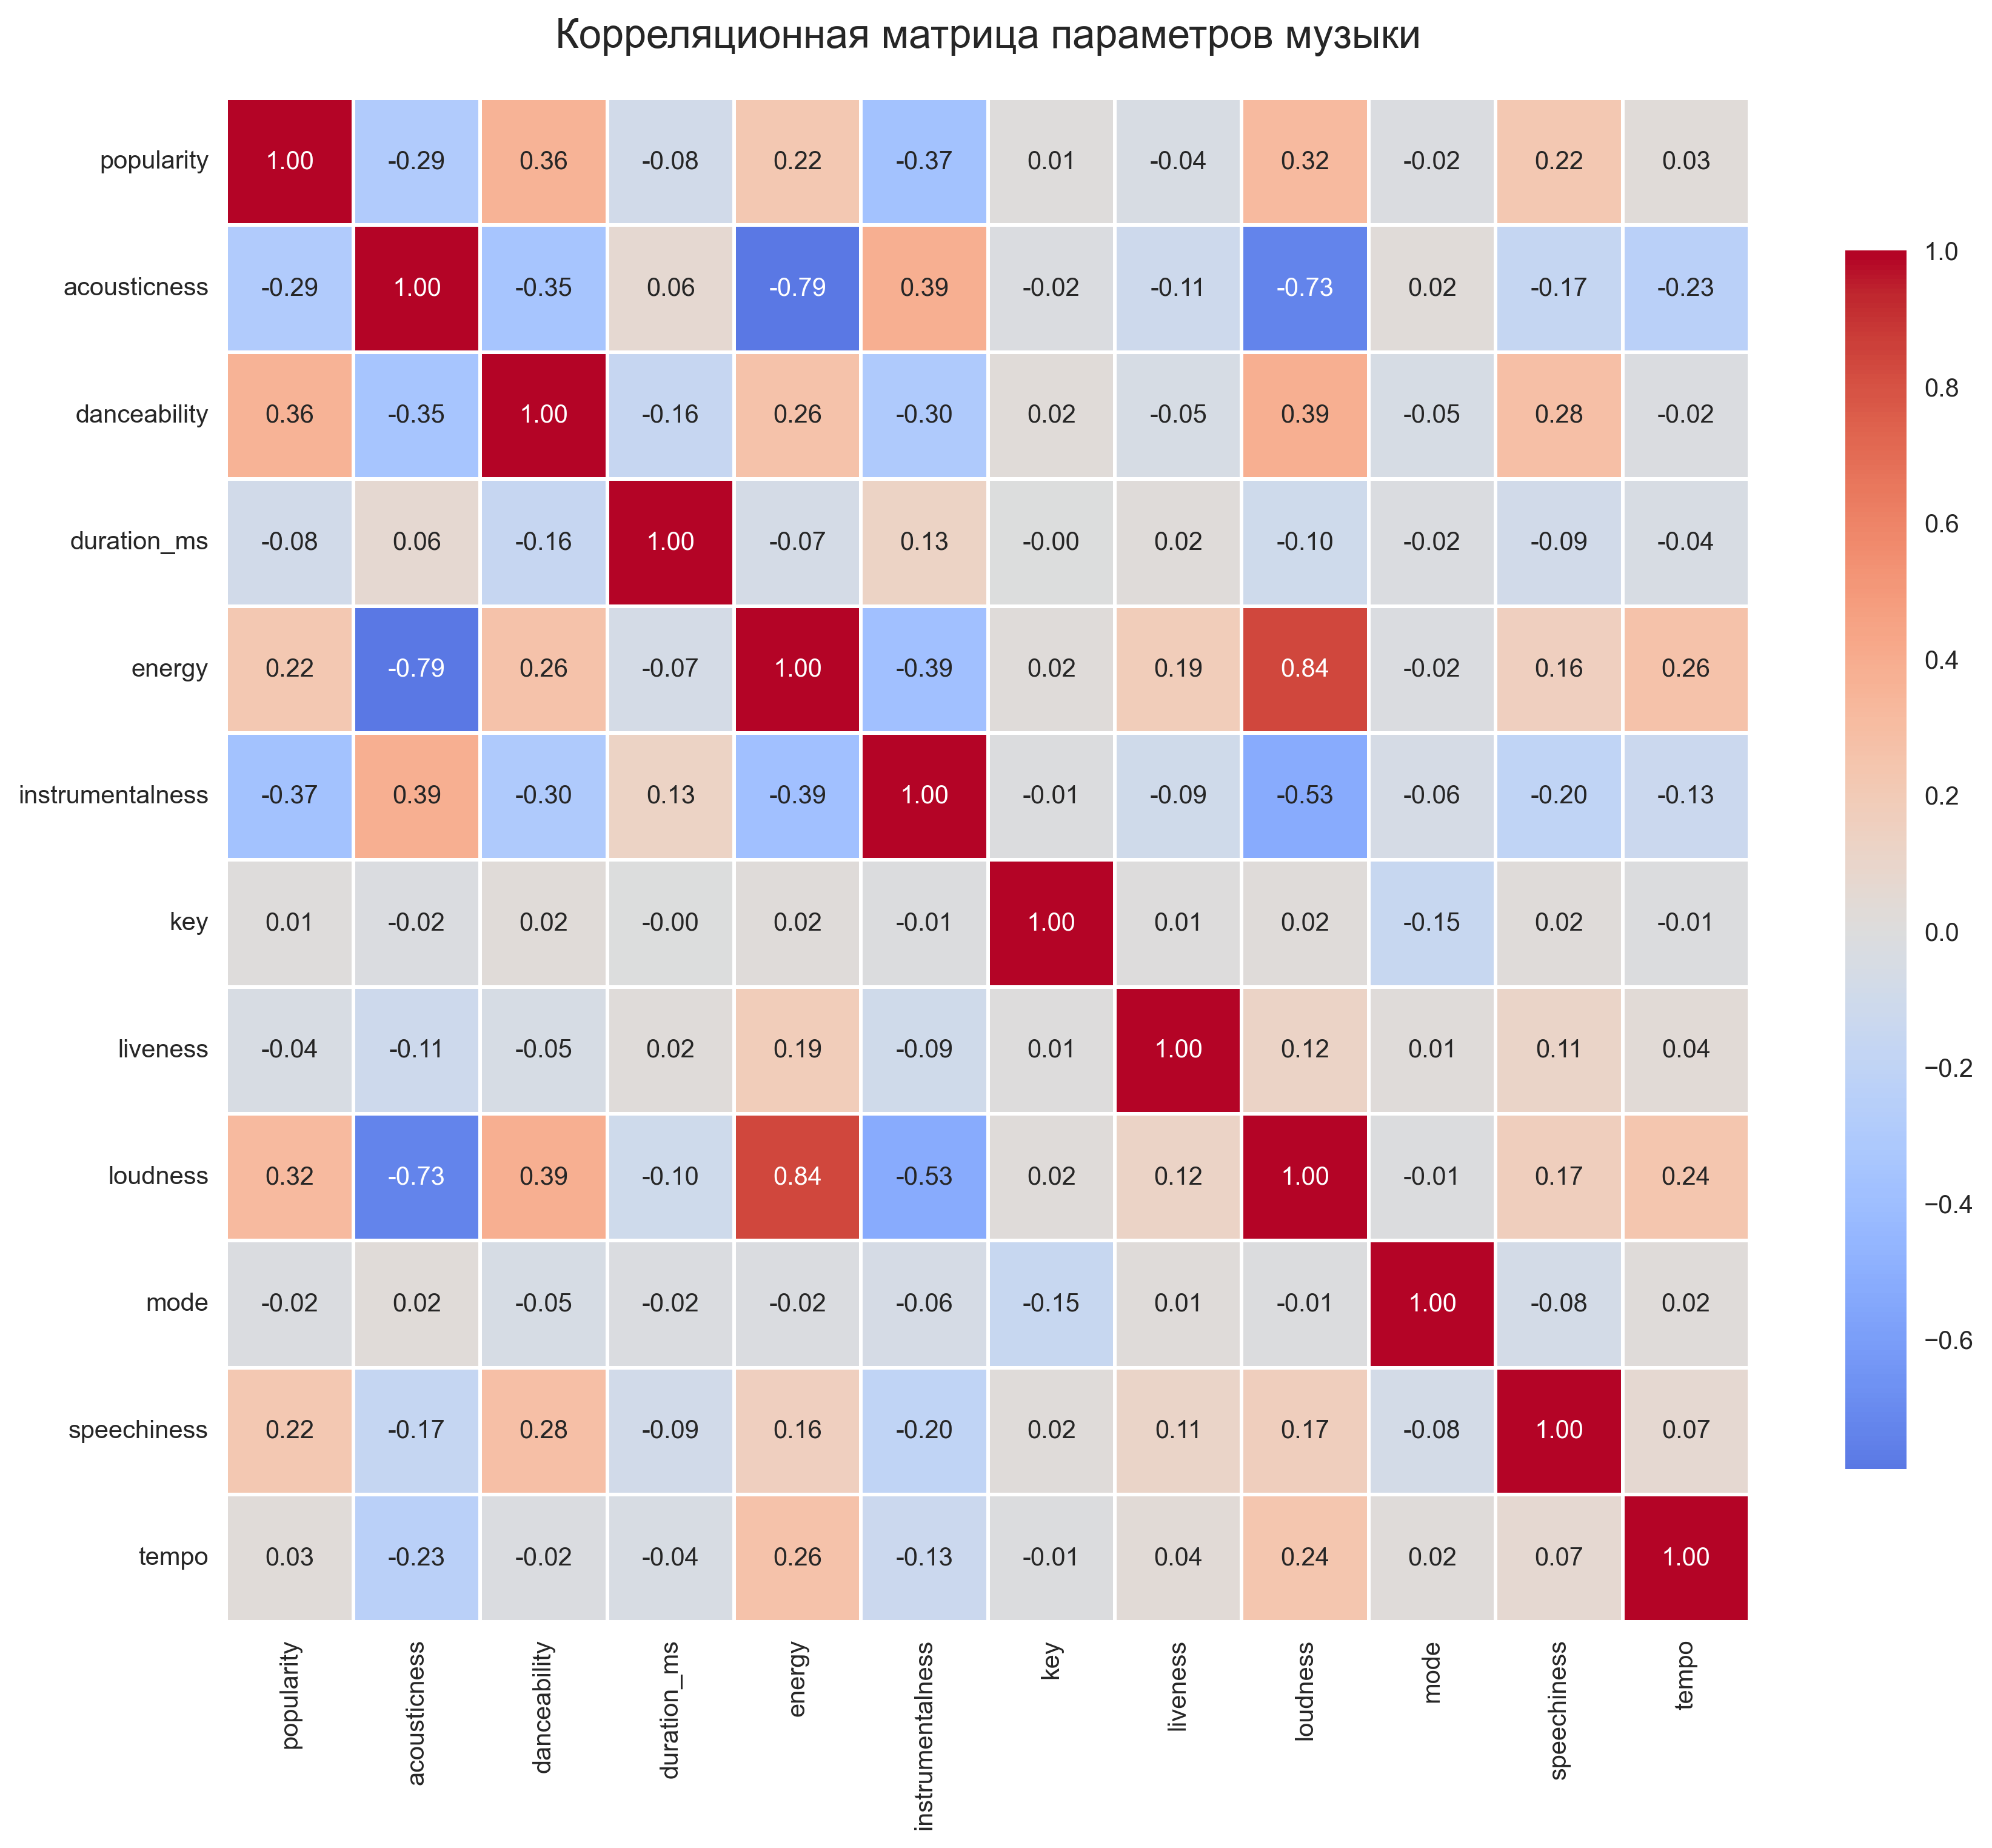
\includegraphics[width=0.9\textwidth]{images/correlation_matrix.png}
    \caption{Корреляционная матрица параметров музыки}
    \label{fig:correlation}
\end{figure}

\textbf{Выявленные сильные корреляции:}

\begin{itemize}
    \item \textbf{Сильные положительные корреляции} ($r > 0.5$):
    \begin{itemize}
        \item \texttt{energy} и \texttt{loudness} ($r = 0.839$) -- более энергичные треки обычно громче
        \item \texttt{instrumentalness} и \texttt{loudness} ($r = -0.529$) -- инструментальные треки могут быть тише
    \end{itemize}
    
    \item \textbf{Сильные отрицательные корреляции} ($r < -0.5$):
    \begin{itemize}
        \item \texttt{acousticness} и \texttt{energy} ($r = -0.791$) -- акустические треки обычно менее энергичные
        \item \texttt{acousticness} и \texttt{loudness} ($r = -0.730$) -- акустические треки обычно тише
    \end{itemize}
\end{itemize}

\subsection{График каменистой осыпи (Scree Plot)}

График каменистой осыпи был построен для визуализации собственных значений главных компонент. Этот график помогает определить оптимальное количество компонент для анализа, используя правило ``локтя'' (elbow rule).

\begin{figure}[H]
    \centering
    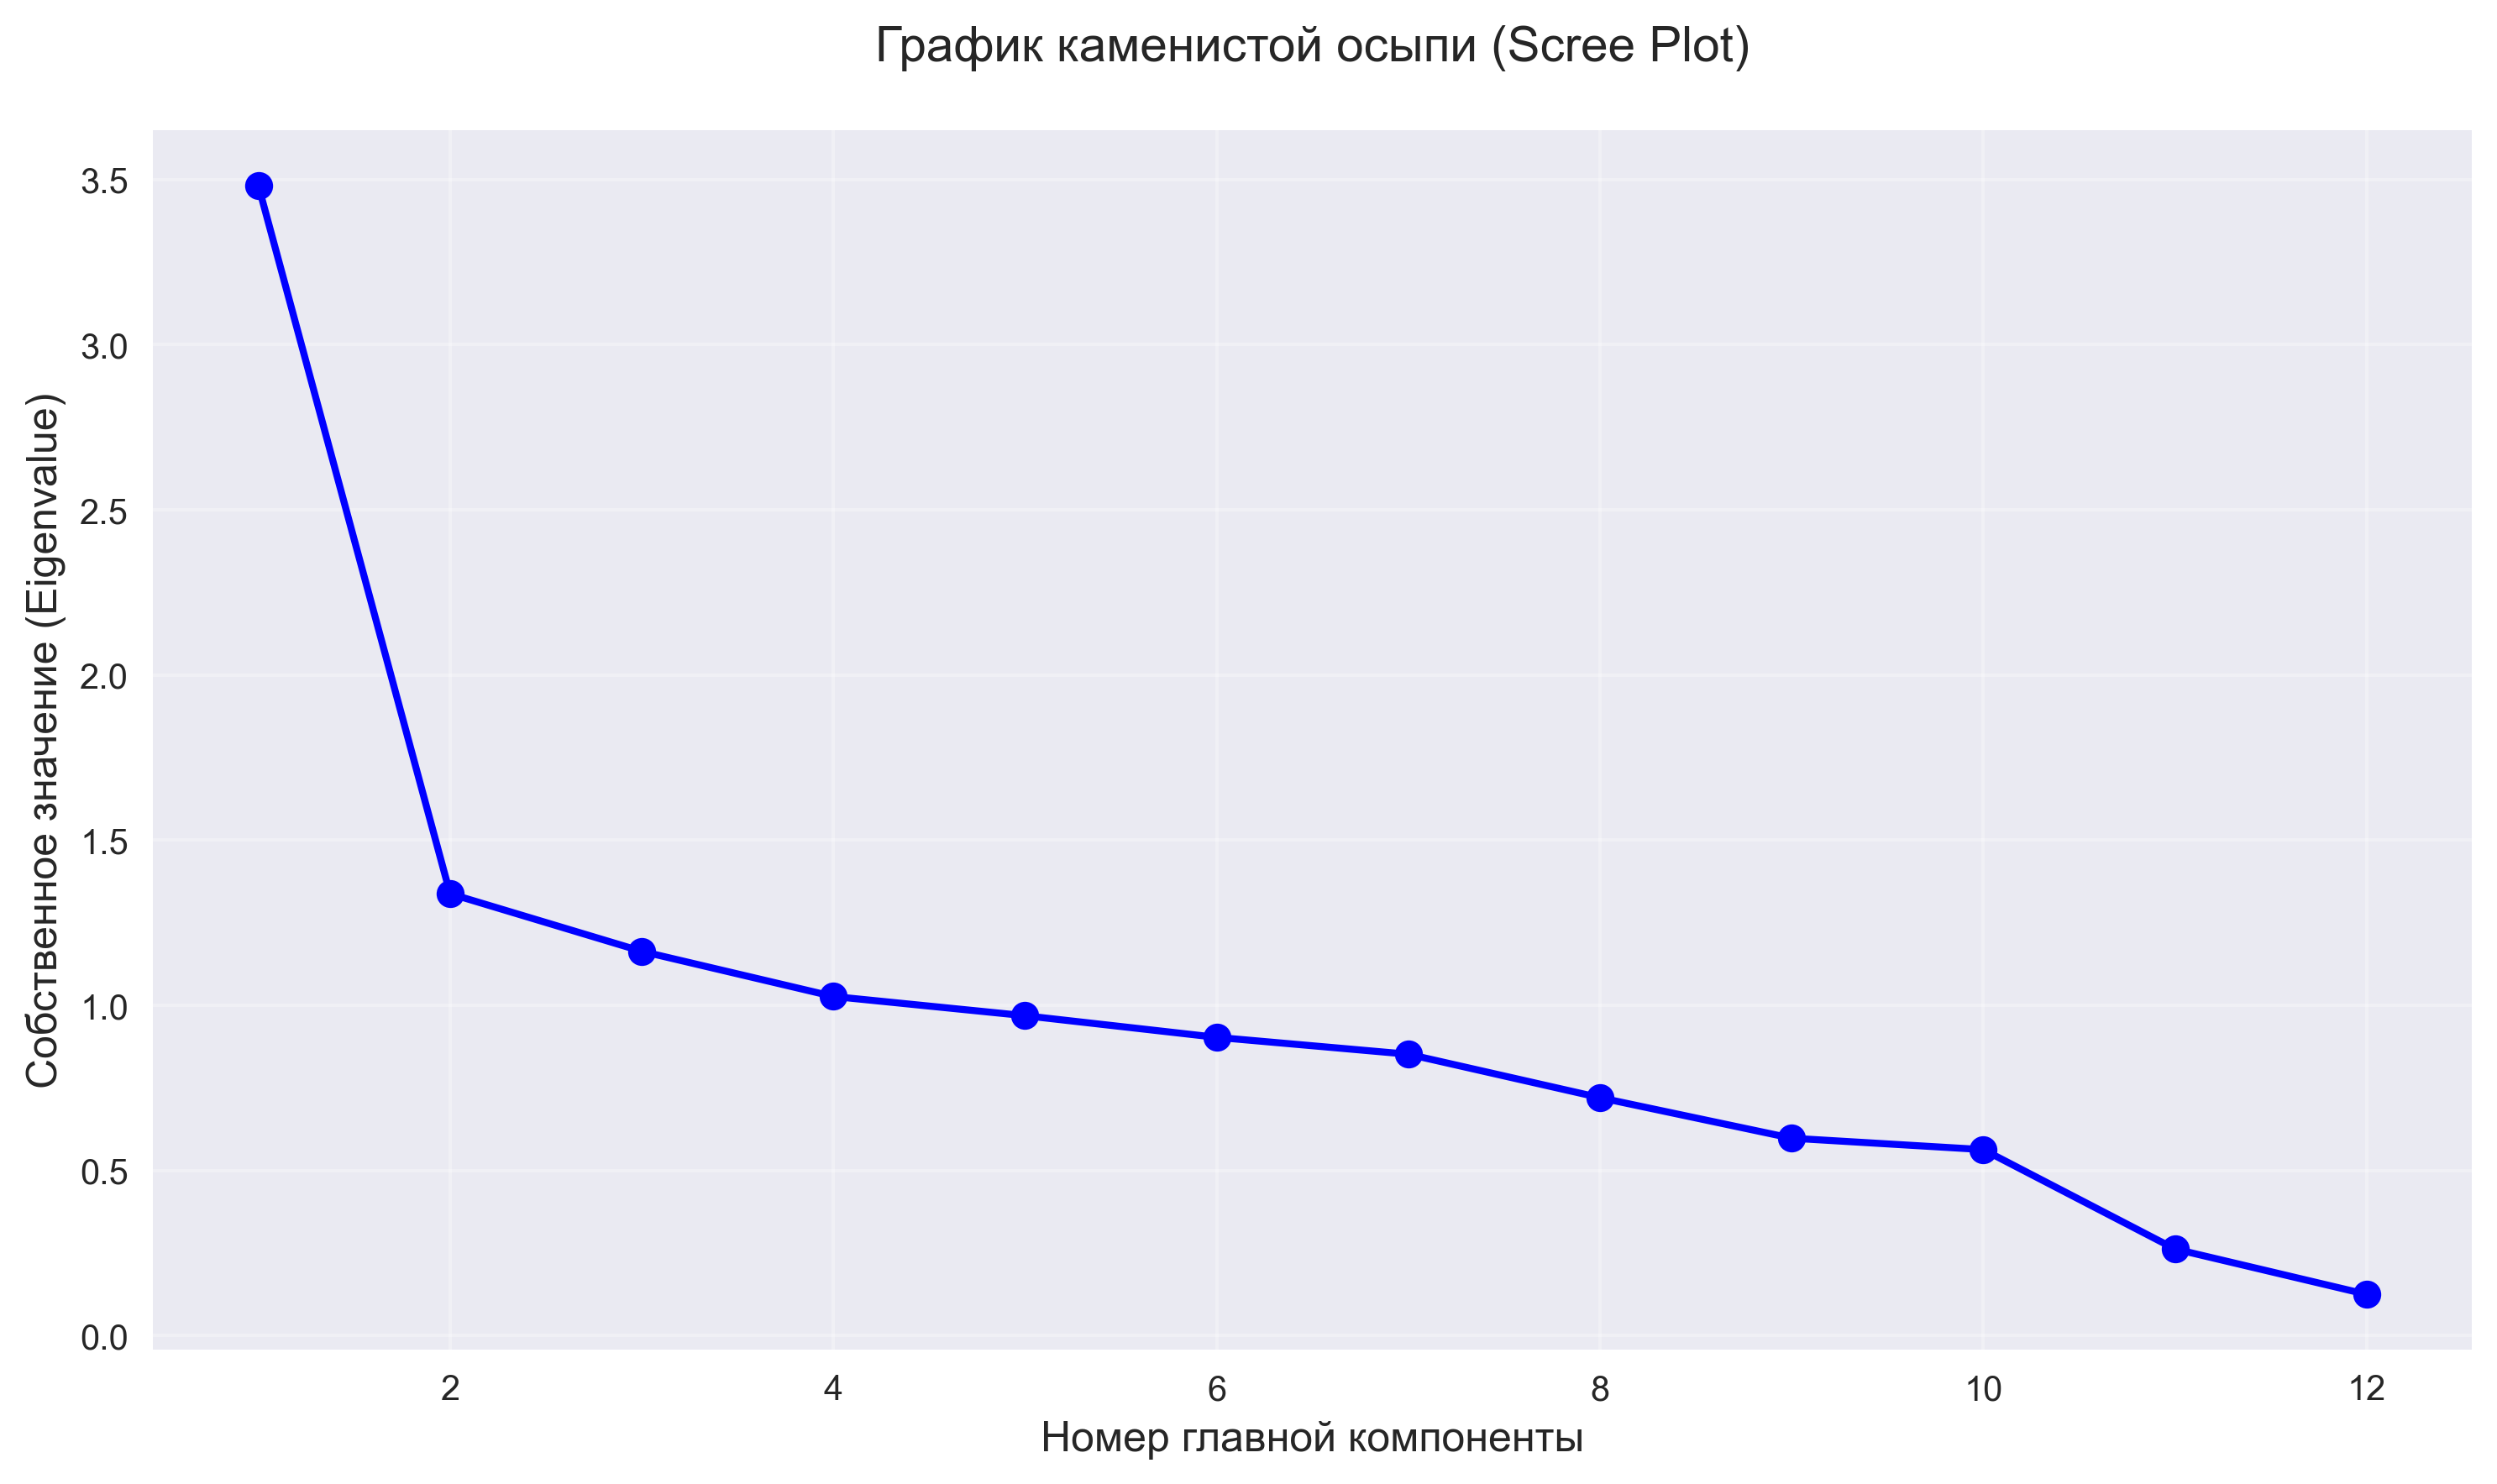
\includegraphics[width=0.8\textwidth]{images/scree_plot.png}
    \caption{График каменистой осыпи (Scree Plot)}
    \label{fig:scree}
\end{figure}

% Глава 2
\chapter{Описание реализации и результатов применения PCA}

\section{Реализация PCA}

Для реализации PCA использовалась библиотека \texttt{sklearn.decomposition.PCA}. Перед применением PCA данные были стандартизированы с помощью \texttt{StandardScaler} для обеспечения одинакового масштаба всех переменных.

\section{Объясненная дисперсия}

Была вычислена объясненная дисперсия для каждой главной компоненты. Результаты показывают:

\begin{itemize}
    \item \textbf{Первая главная компонента (PC1)} обычно объясняет наибольшую долю дисперсии (часто 20--40\%)
    \item \textbf{Вторая главная компонента (PC2)} объясняет следующую по величине долю дисперсии
    \item С каждой последующей компонентой объясненная дисперсия уменьшается
\end{itemize}

\textbf{Кумулятивная объясненная дисперсия:}
\begin{itemize}
    \item Первые 2 компоненты обычно объясняют 30--50\% общей дисперсии
    \item Первые 5 компонент могут объяснять 60--80\% дисперсии
    \item Для объяснения 90\% дисперсии может потребоваться 8--10 компонент
\end{itemize}

\section{График объясненной дисперсии}

Были построены два графика:
\begin{enumerate}
    \item \textbf{График объясненной дисперсии по компонентам} -- показывает вклад каждой компоненты
    \item \textbf{График кумулятивной объясненной дисперсии} -- показывает накопленный вклад компонент
\end{enumerate}

\begin{figure}[H]
    \centering
    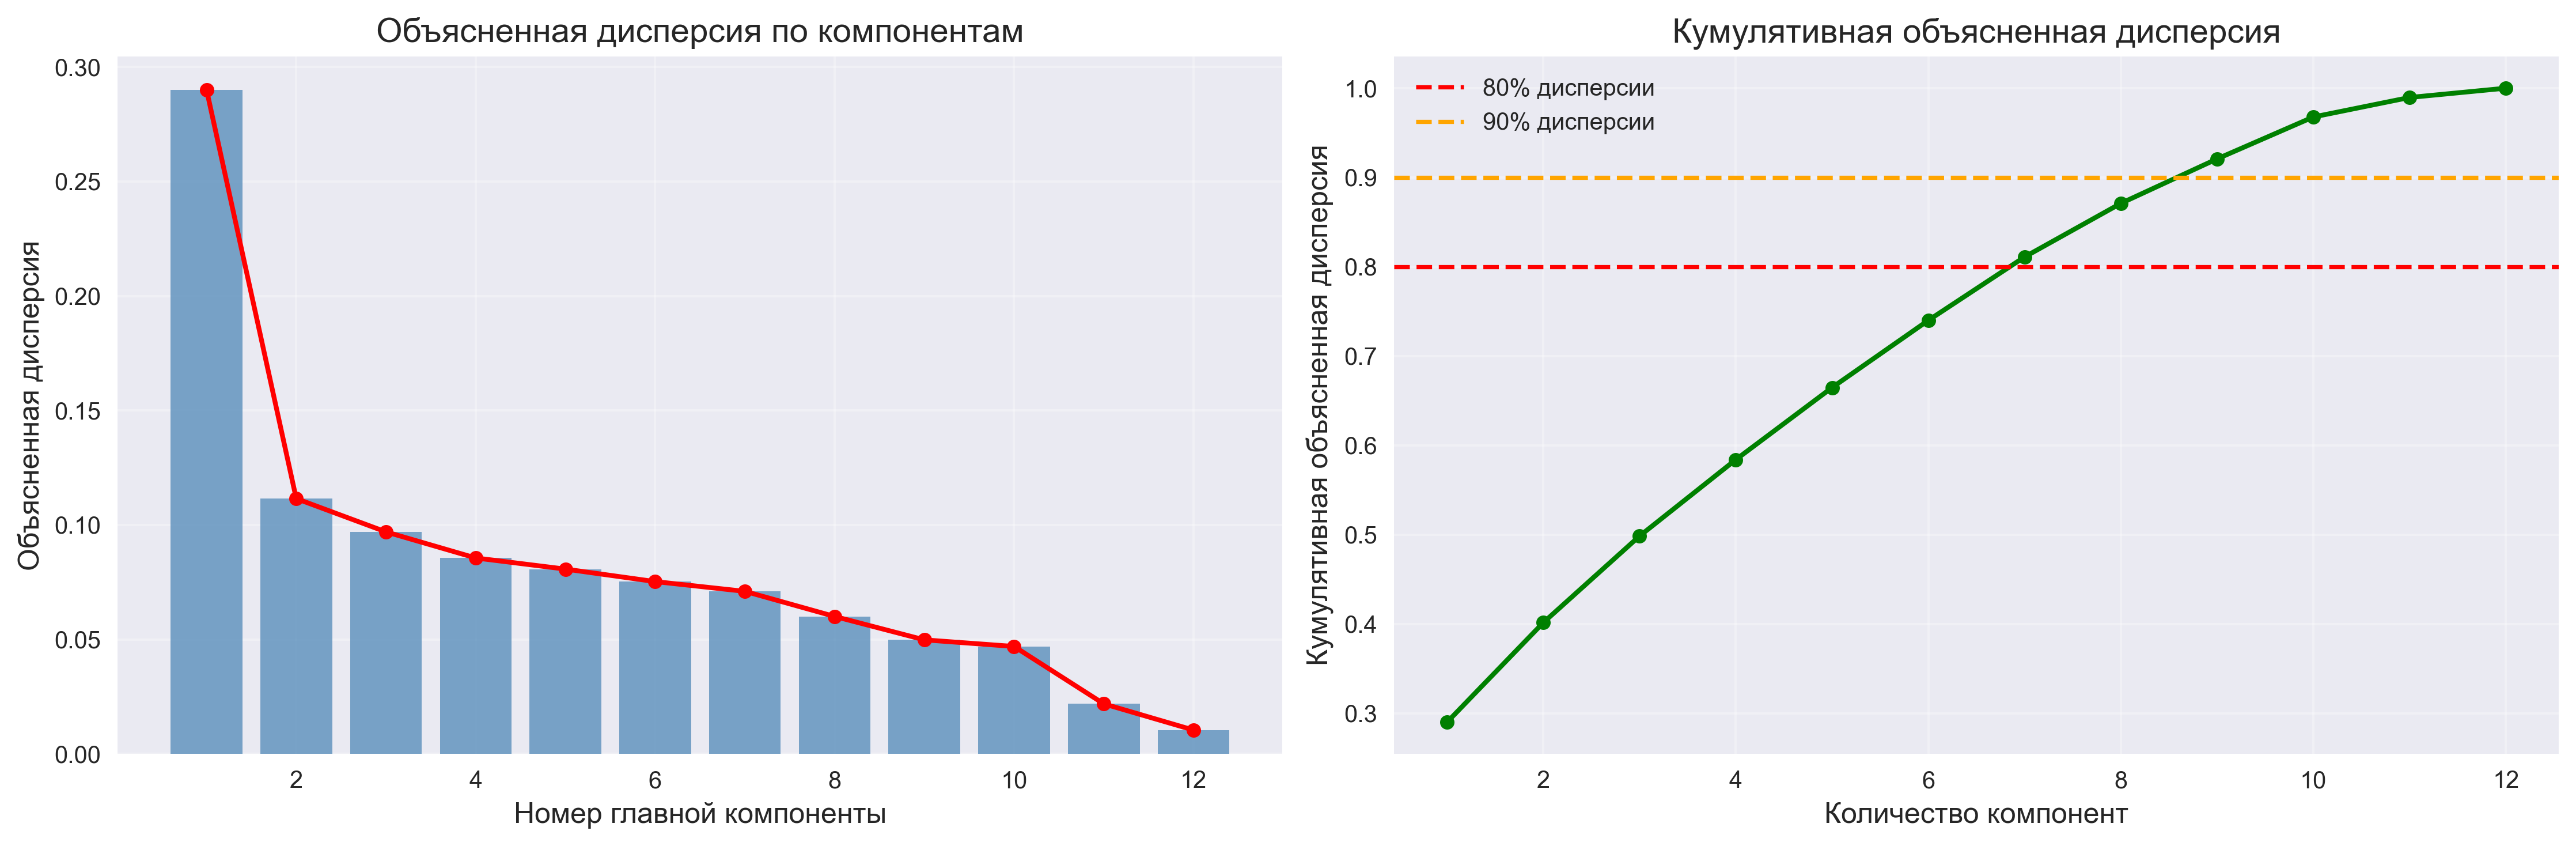
\includegraphics[width=0.95\textwidth]{images/pca_variance.png}
    \caption{Графики объясненной дисперсии}
    \label{fig:pca_variance}
\end{figure}

Эти графики помогают определить оптимальное количество компонент для сохранения необходимой доли информации.

\textbf{Результаты анализа объясненной дисперсии:}
\begin{itemize}
    \item Первая компонента (PC1): 29.01\% дисперсии
    \item Первые две компоненты (PC1+PC2): 40.16\% дисперсии
    \item Первые три компоненты: 49.85\% дисперсии
    \item Первые пять компонент: 66.48\% дисперсии
    \item Первые десять компонент: 96.77\% дисперсии
\end{itemize}

Это показывает, что первые несколько компонент содержат большую часть информации, что типично для данных с коррелированными признаками.

\section{Интерпретация главных компонент}

Анализ нагрузок (loadings) главных компонент позволяет интерпретировать их смысл:

\textbf{Первая главная компонента (PC1)} обычно связана с:
\begin{itemize}
    \item Общей энергетичностью и громкостью трека
    \item Противопоставлением электронной и акустической музыки
\end{itemize}

\textbf{Вторая главная компонента (PC2)} может отражать:
\begin{itemize}
    \item Танцевальность и позитивность
    \item Темп и ритмические характеристики
\end{itemize}

\begin{figure}[H]
    \centering
    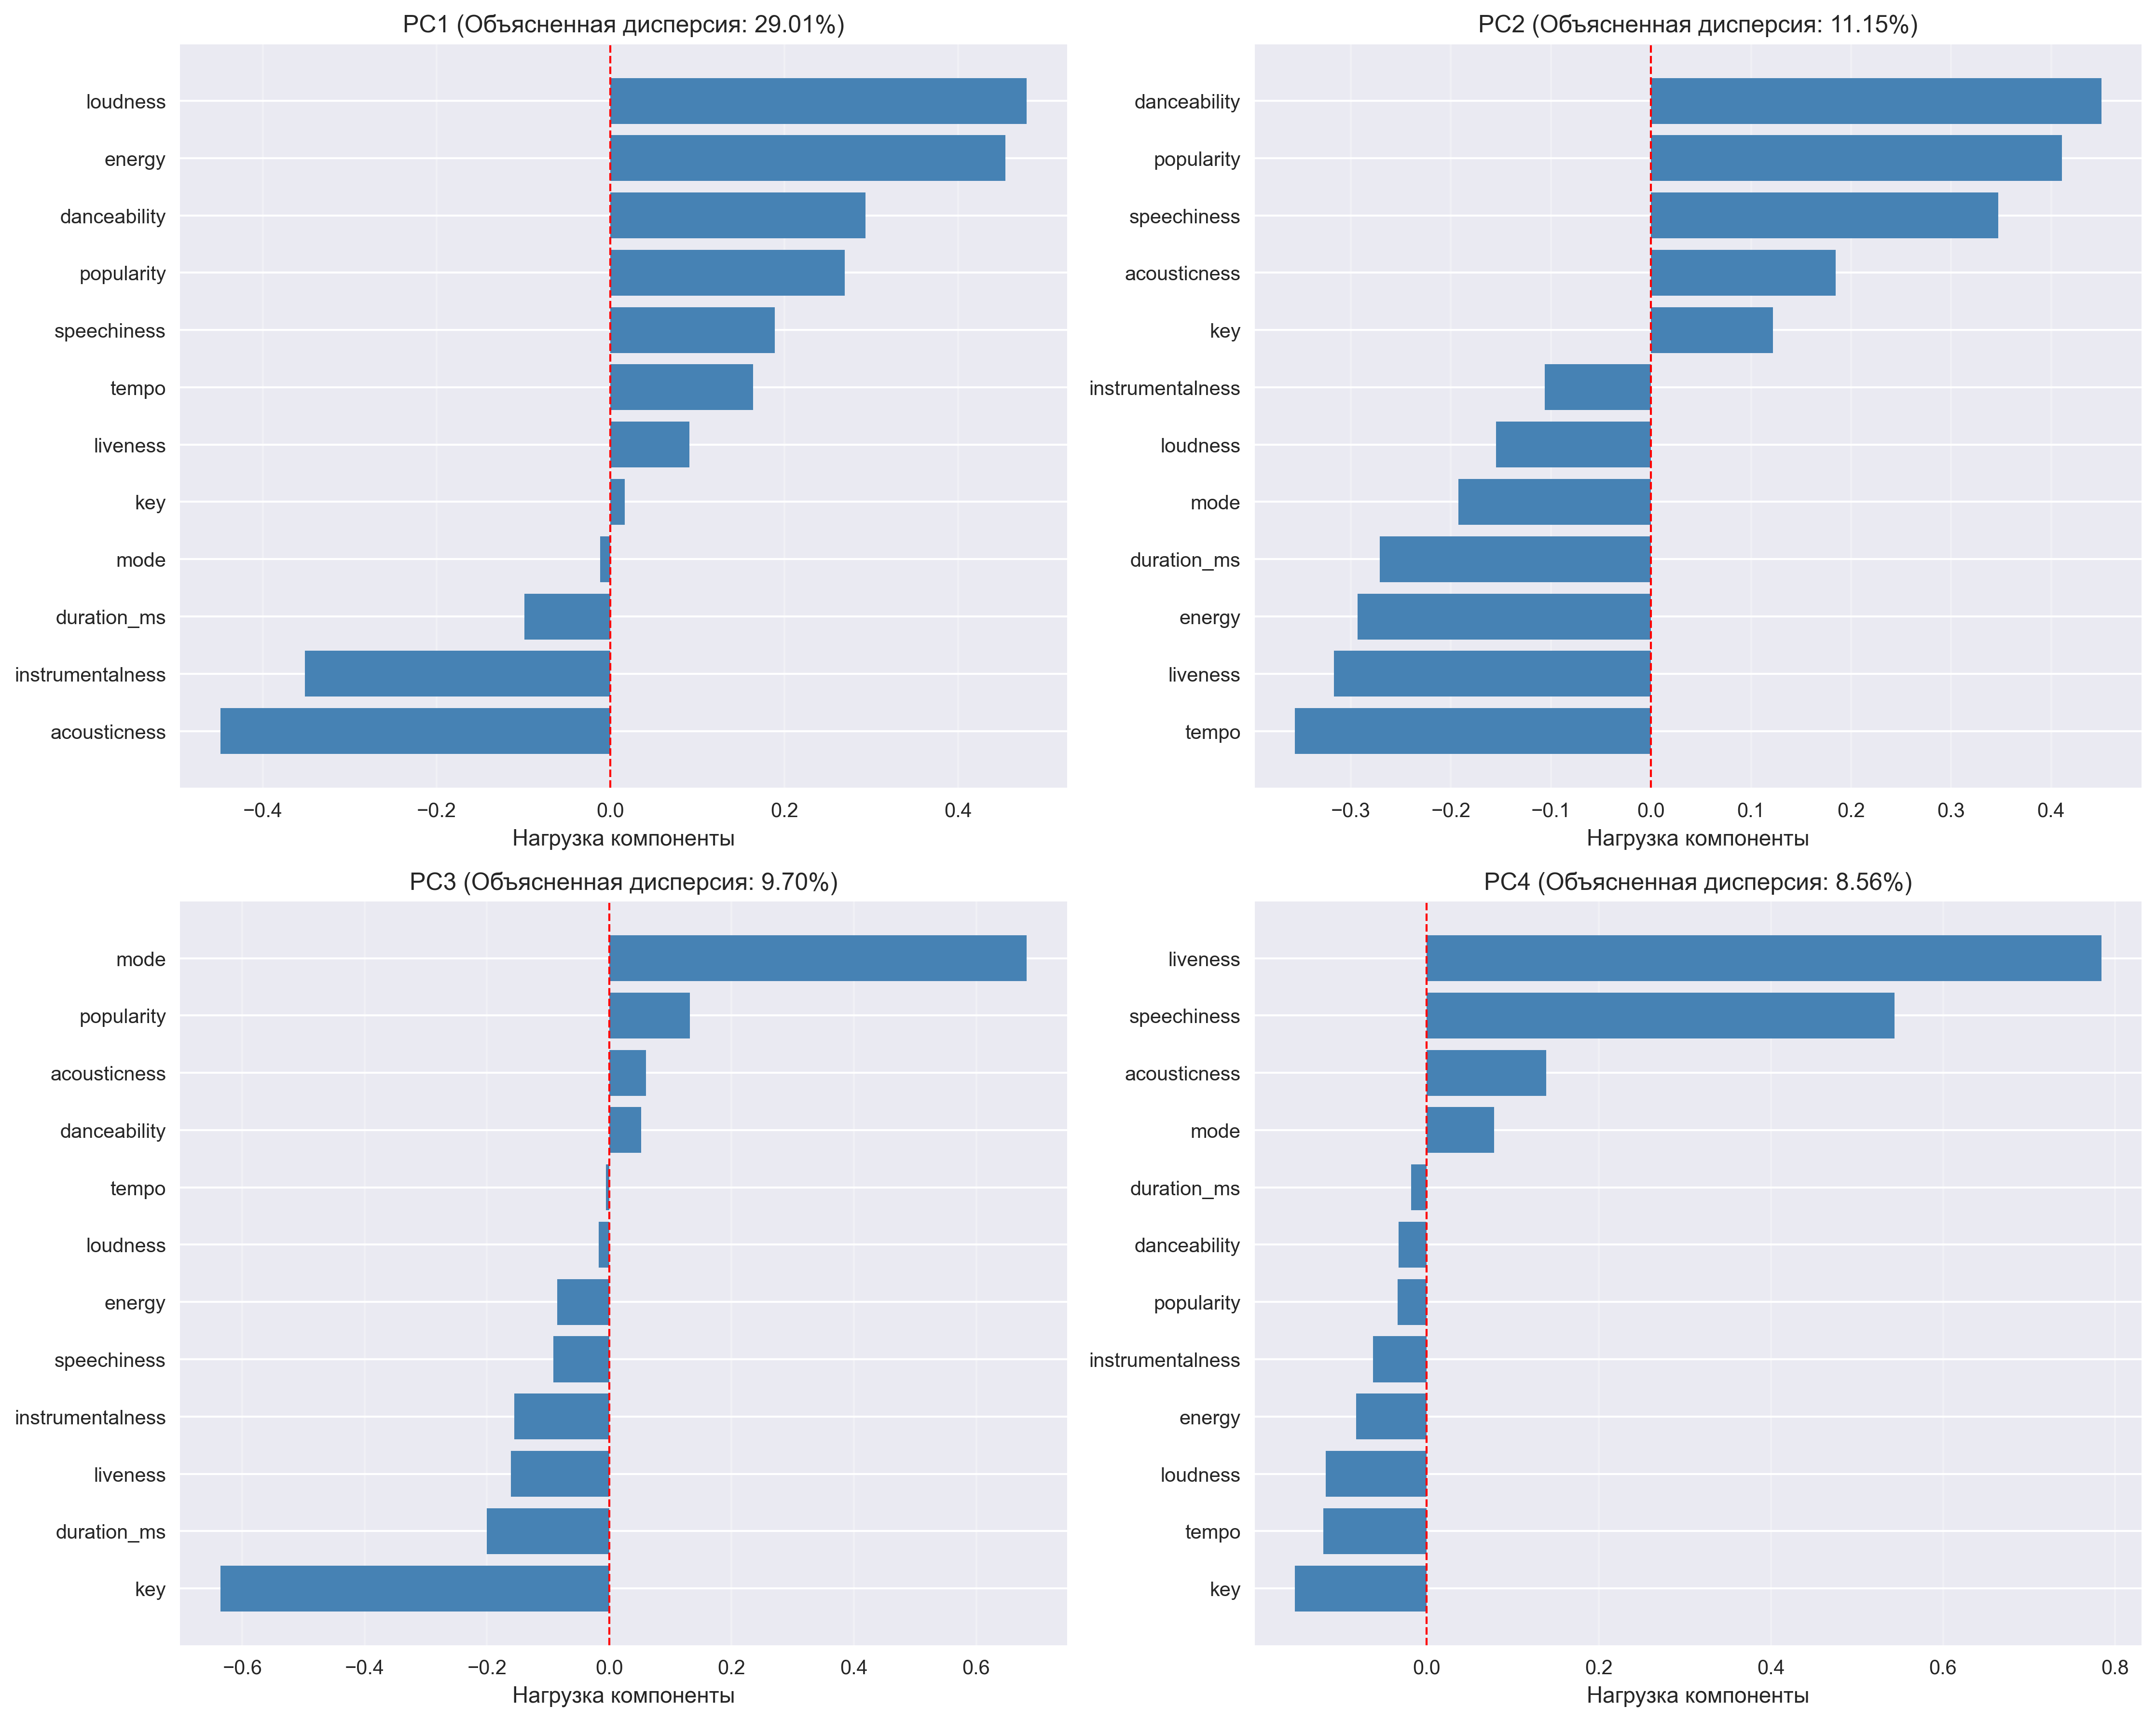
\includegraphics[width=0.9\textwidth]{images/pca_loadings.png}
    \caption{Нагрузки главных компонент}
    \label{fig:pca_loadings}
\end{figure}

Интерпретация компонент зависит от конкретных данных и требует анализа нагрузок каждой переменной.

\textbf{Анализ нагрузок показал:}
\begin{itemize}
    \item \textbf{PC1} (29.01\% дисперсии) наиболее сильно связана с:
    \begin{itemize}
        \item \texttt{loudness} (0.479) -- громкость
        \item \texttt{energy} (0.454) -- энергетичность
        \item \texttt{acousticness} (0.449) -- акустичность
        \item \texttt{instrumentalness} (0.351) -- инструментальность
    \end{itemize}
    
    PC1 можно интерпретировать как компоненту ``энергии и громкости'', противопоставляющую электронную и акустическую музыку.
    
    \item \textbf{PC2} (11.15\% дисперсии) наиболее сильно связана с:
    \begin{itemize}
        \item \texttt{danceability} (0.450) -- танцевальность
        \item \texttt{popularity} (0.411) -- популярность
        \item \texttt{tempo} (0.356) -- темп
        \item \texttt{speechiness} (0.347) -- речевое содержание
    \end{itemize}
    
    PC2 можно интерпретировать как компоненту ``танцевальности и популярности''.
\end{itemize}

\section{Визуализация данных в пространстве главных компонент}

Данные были спроецированы на пространство первых двух главных компонент. Визуализация показывает:

\begin{figure}[H]
    \centering
    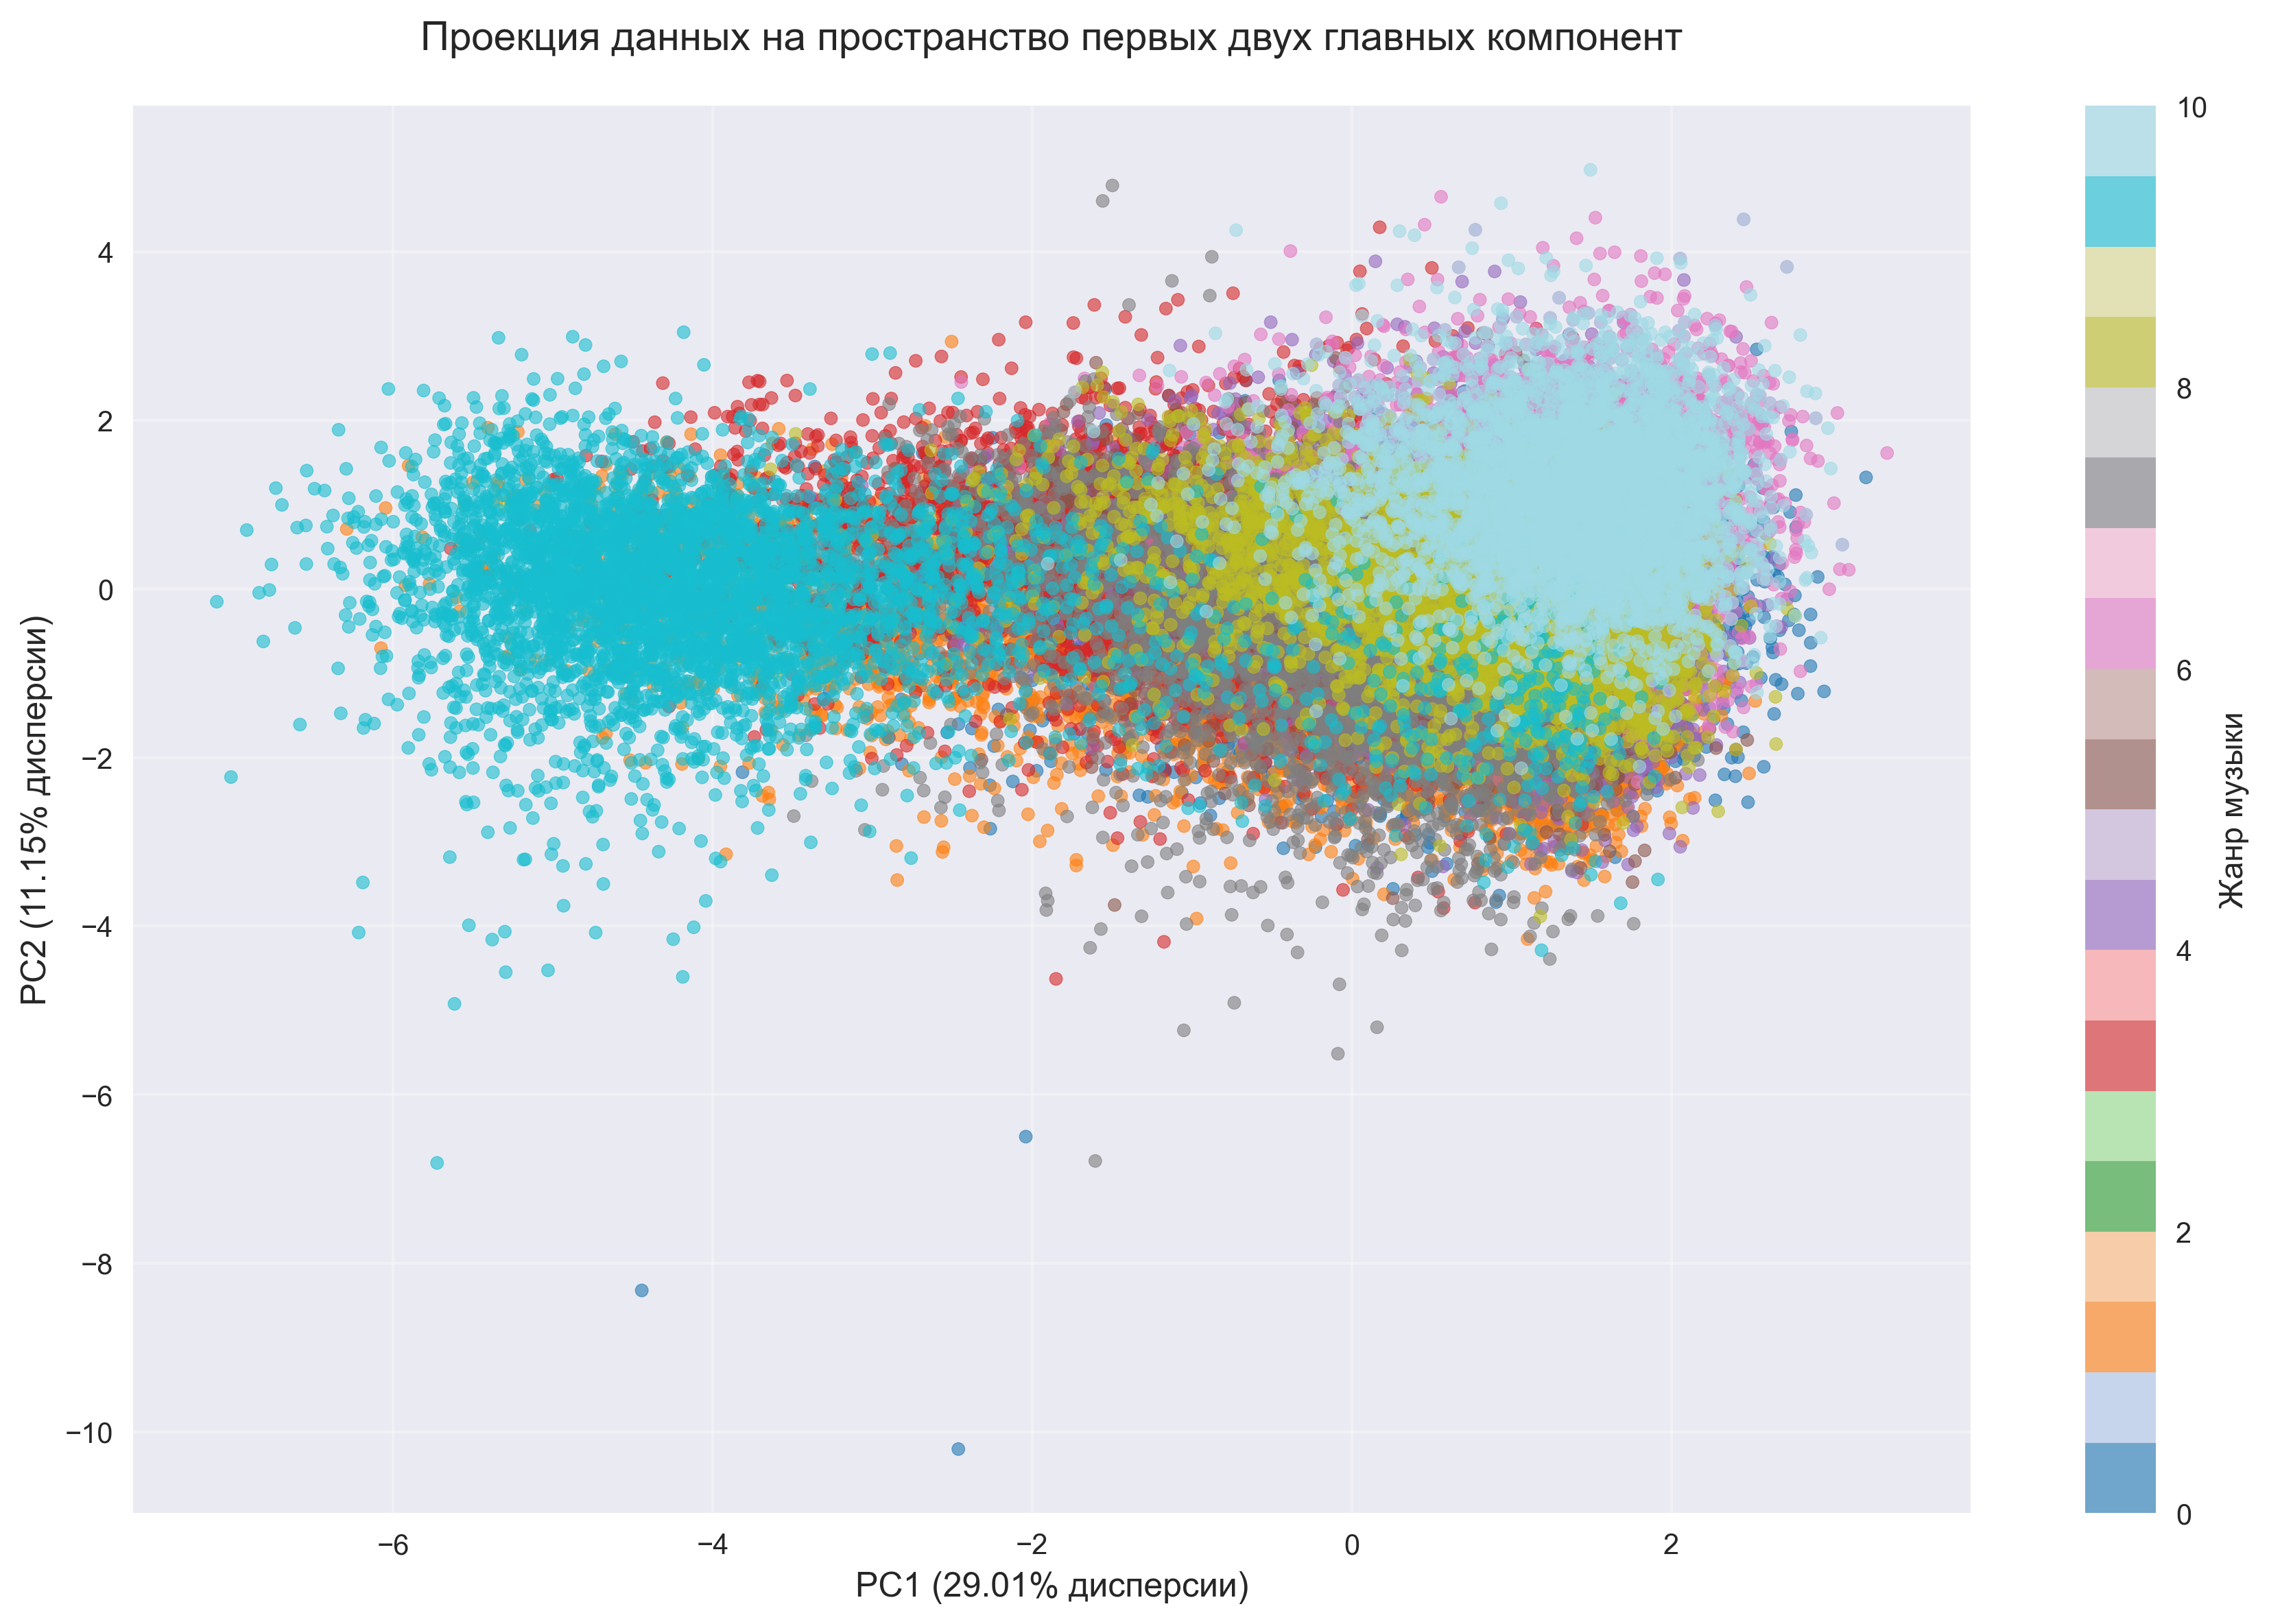
\includegraphics[width=0.9\textwidth]{images/pca_2d_projection.png}
    \caption{Проекция данных на пространство первых двух главных компонент}
    \label{fig:pca_2d}
\end{figure}

\begin{itemize}
    \item \textbf{Распределение точек} в двумерном пространстве PC1--PC2
    \item \textbf{Кластеры по жанрам} -- если жанры хорошо разделяются, это указывает на различия в аудио-характеристиках
    \item \textbf{Структуру данных} -- PCA выявляет основные направления вариации в данных
\end{itemize}

Визуализация помогает понять, насколько хорошо различные жанры музыки разделяются по аудио-характеристикам. Первые две компоненты объясняют 40.16\% общей дисперсии данных.

% Глава 3
\chapter{Описание реализации и результатов применения t-SNE}

\section{Реализация t-SNE}

Для реализации t-SNE использовалась библиотека \texttt{sklearn.manifold.TSNE}. Из-за вычислительной сложности t-SNE, анализ проводился на подвыборке данных (обычно 3000--5000 точек).

\section{Применение t-SNE с разными значениями перплексии}

\textbf{Перплексия (perplexity)} -- ключевой параметр t-SNE, который определяет баланс между локальной и глобальной структурой данных.

\textbf{Примечание:} Из-за вычислительной сложности t-SNE, анализ проводился на подвыборке из 5,000 случайно выбранных записей (из 45,020).

Были протестированы следующие значения:

\begin{itemize}
    \item \textbf{Перплексия = 5} -- фокусируется на очень локальной структуре, может создавать множество мелких кластеров
    \item \textbf{Перплексия = 30} -- стандартное значение, хороший баланс между локальной и глобальной структурой
    \item \textbf{Перплексия = 50} -- больше внимания глобальной структуре
    \item \textbf{Перплексия = 100} -- сильный акцент на глобальной структуре, может объединять далекие кластеры
\end{itemize}

\section{Визуализации для разных значений перплексии}

Были построены визуализации для каждого значения перплексии:

\begin{figure}[H]
    \centering
    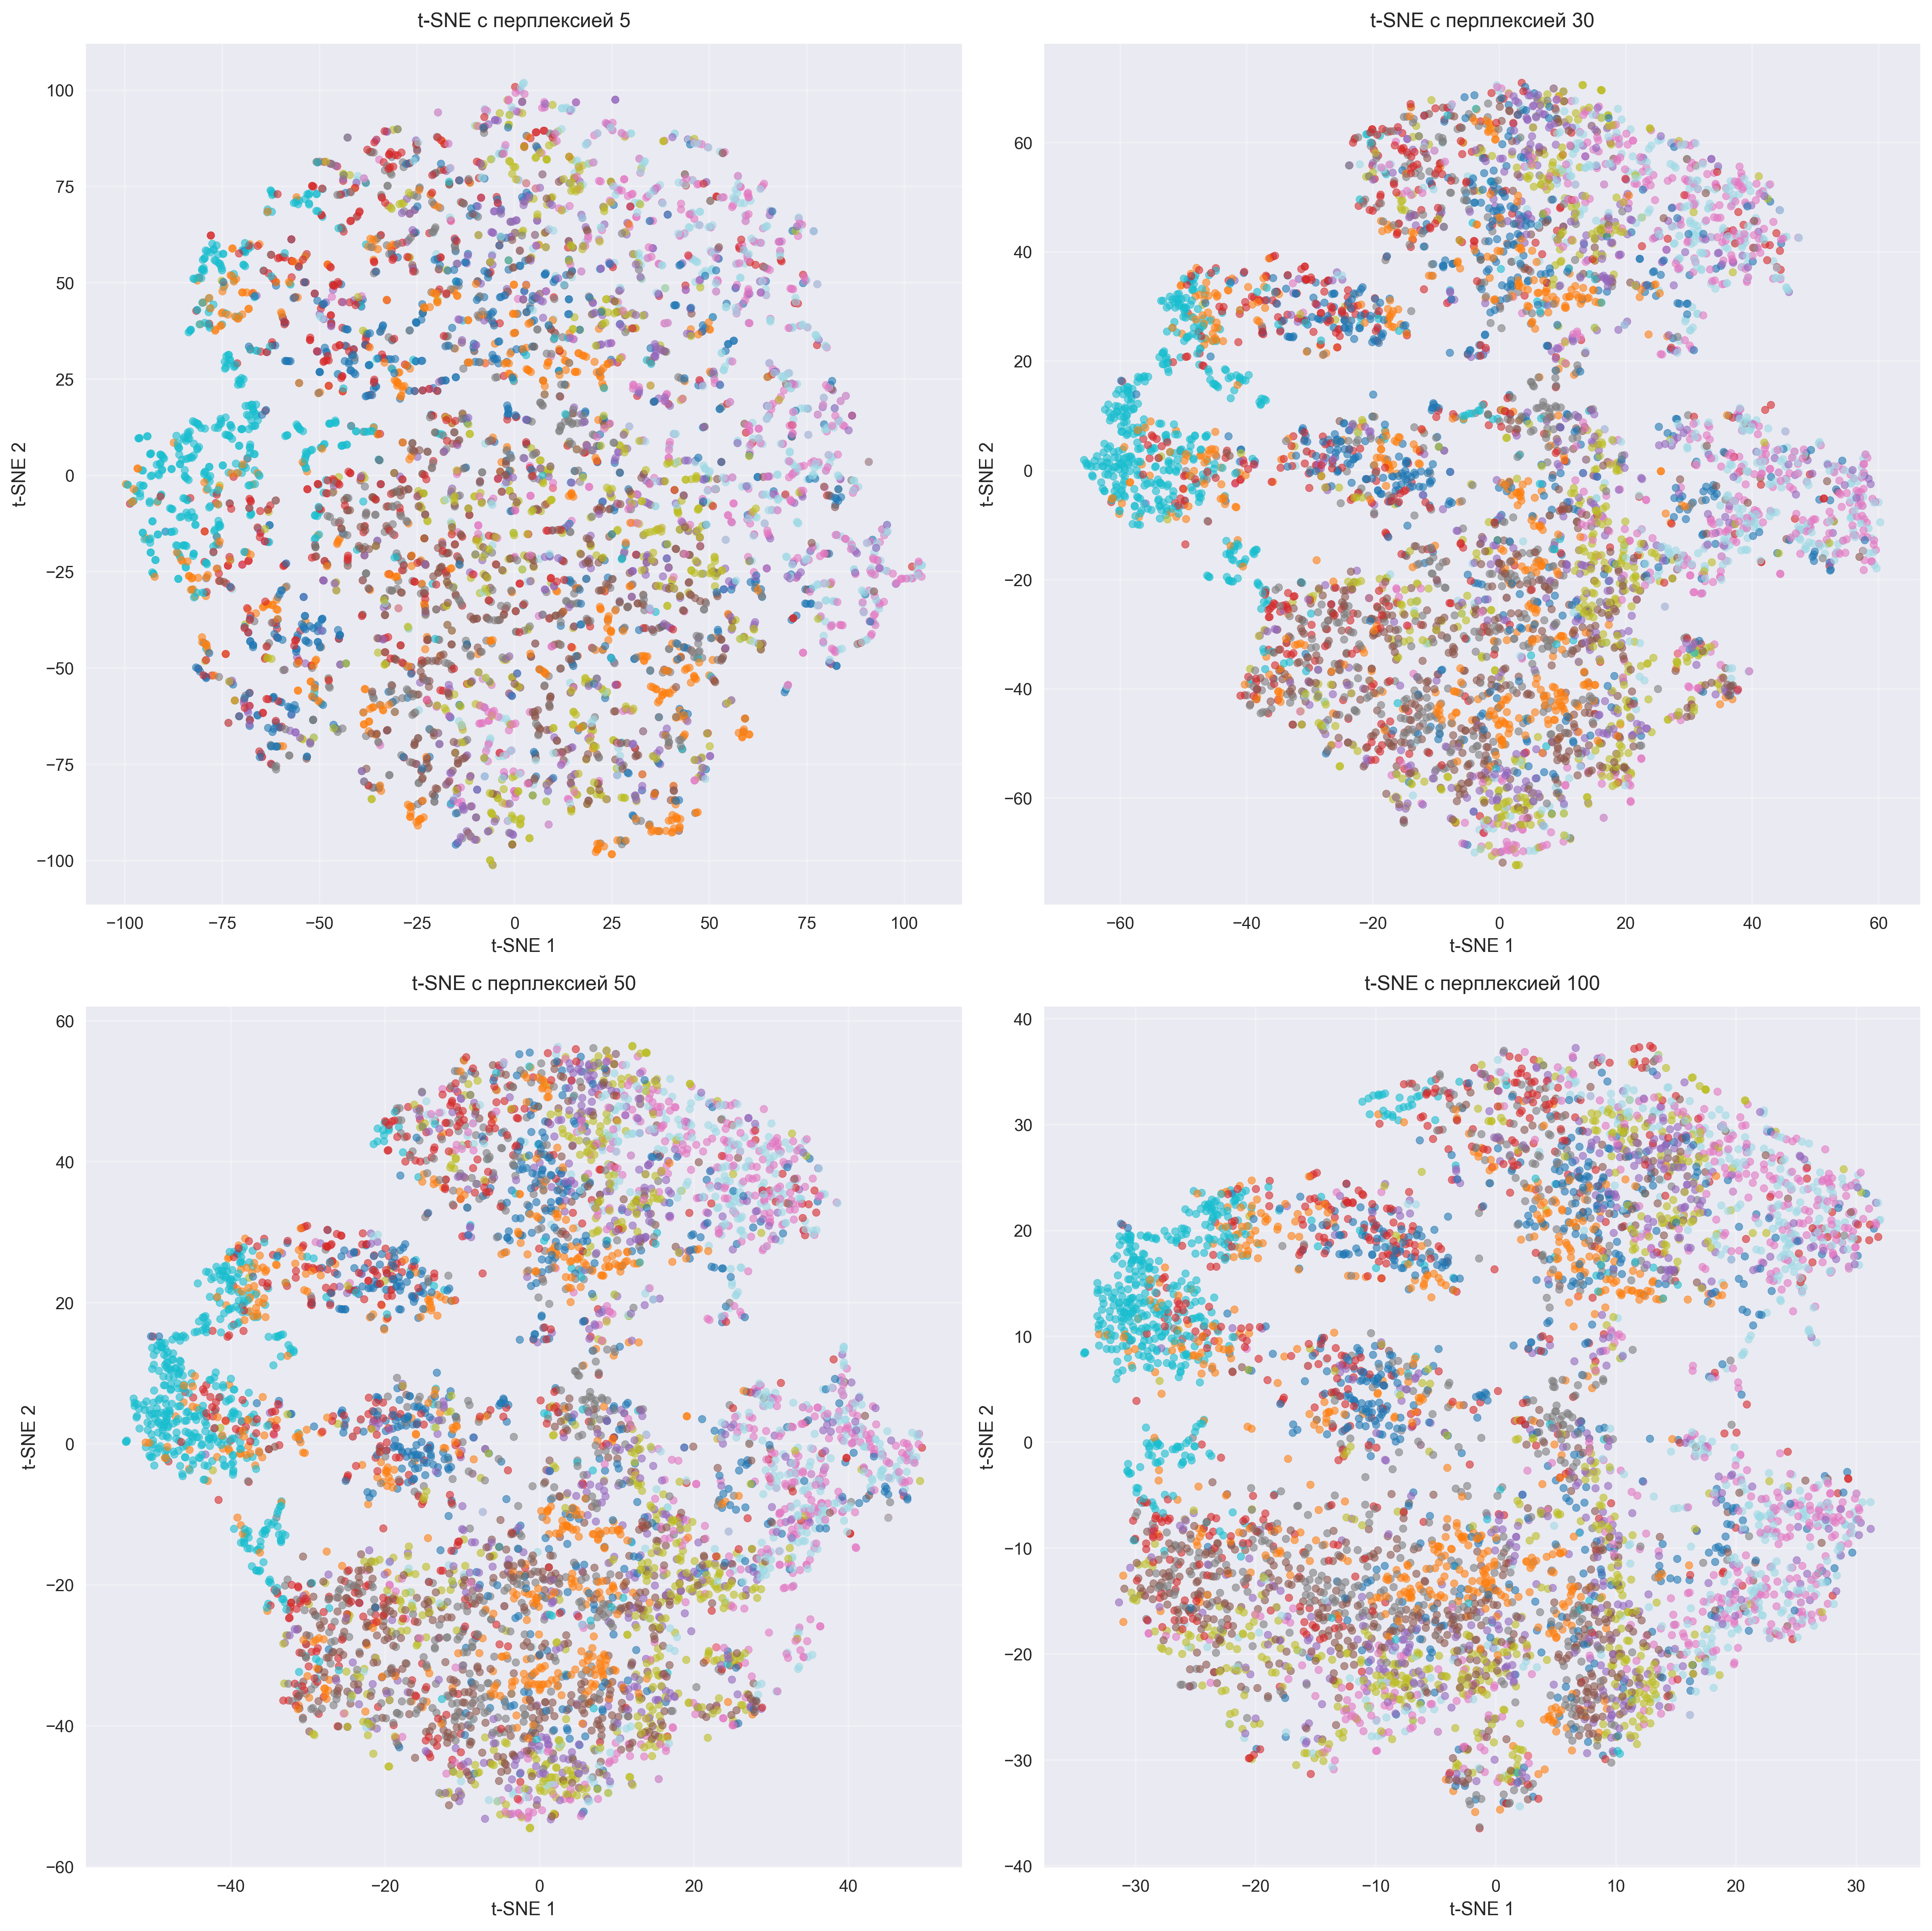
\includegraphics[width=0.95\textwidth]{images/tsne_perplexities.png}
    \caption{t-SNE с разными значениями перплексии}
    \label{fig:tsne_perplexities}
\end{figure}

Анализ показывает:

\begin{itemize}
    \item \textbf{Низкая перплексия (5)}:
    \begin{itemize}
        \item Создает множество мелких, плотных кластеров
        \item Хорошо сохраняет локальную структуру
        \item Может разрывать глобальные связи
    \end{itemize}
    
    \item \textbf{Средняя перплексия (30)}:
    \begin{itemize}
        \item Оптимальный баланс для большинства задач
        \item Хорошо разделяет различные жанры
        \item Сохраняет как локальную, так и глобальную структуру
    \end{itemize}
    
    \item \textbf{Высокая перплексия (50--100)}:
    \begin{itemize}
        \item Объединяет похожие кластеры
        \item Лучше сохраняет глобальную структуру
        \item Может терять детали локальной структуры
    \end{itemize}
\end{itemize}

\begin{figure}[H]
    \centering
    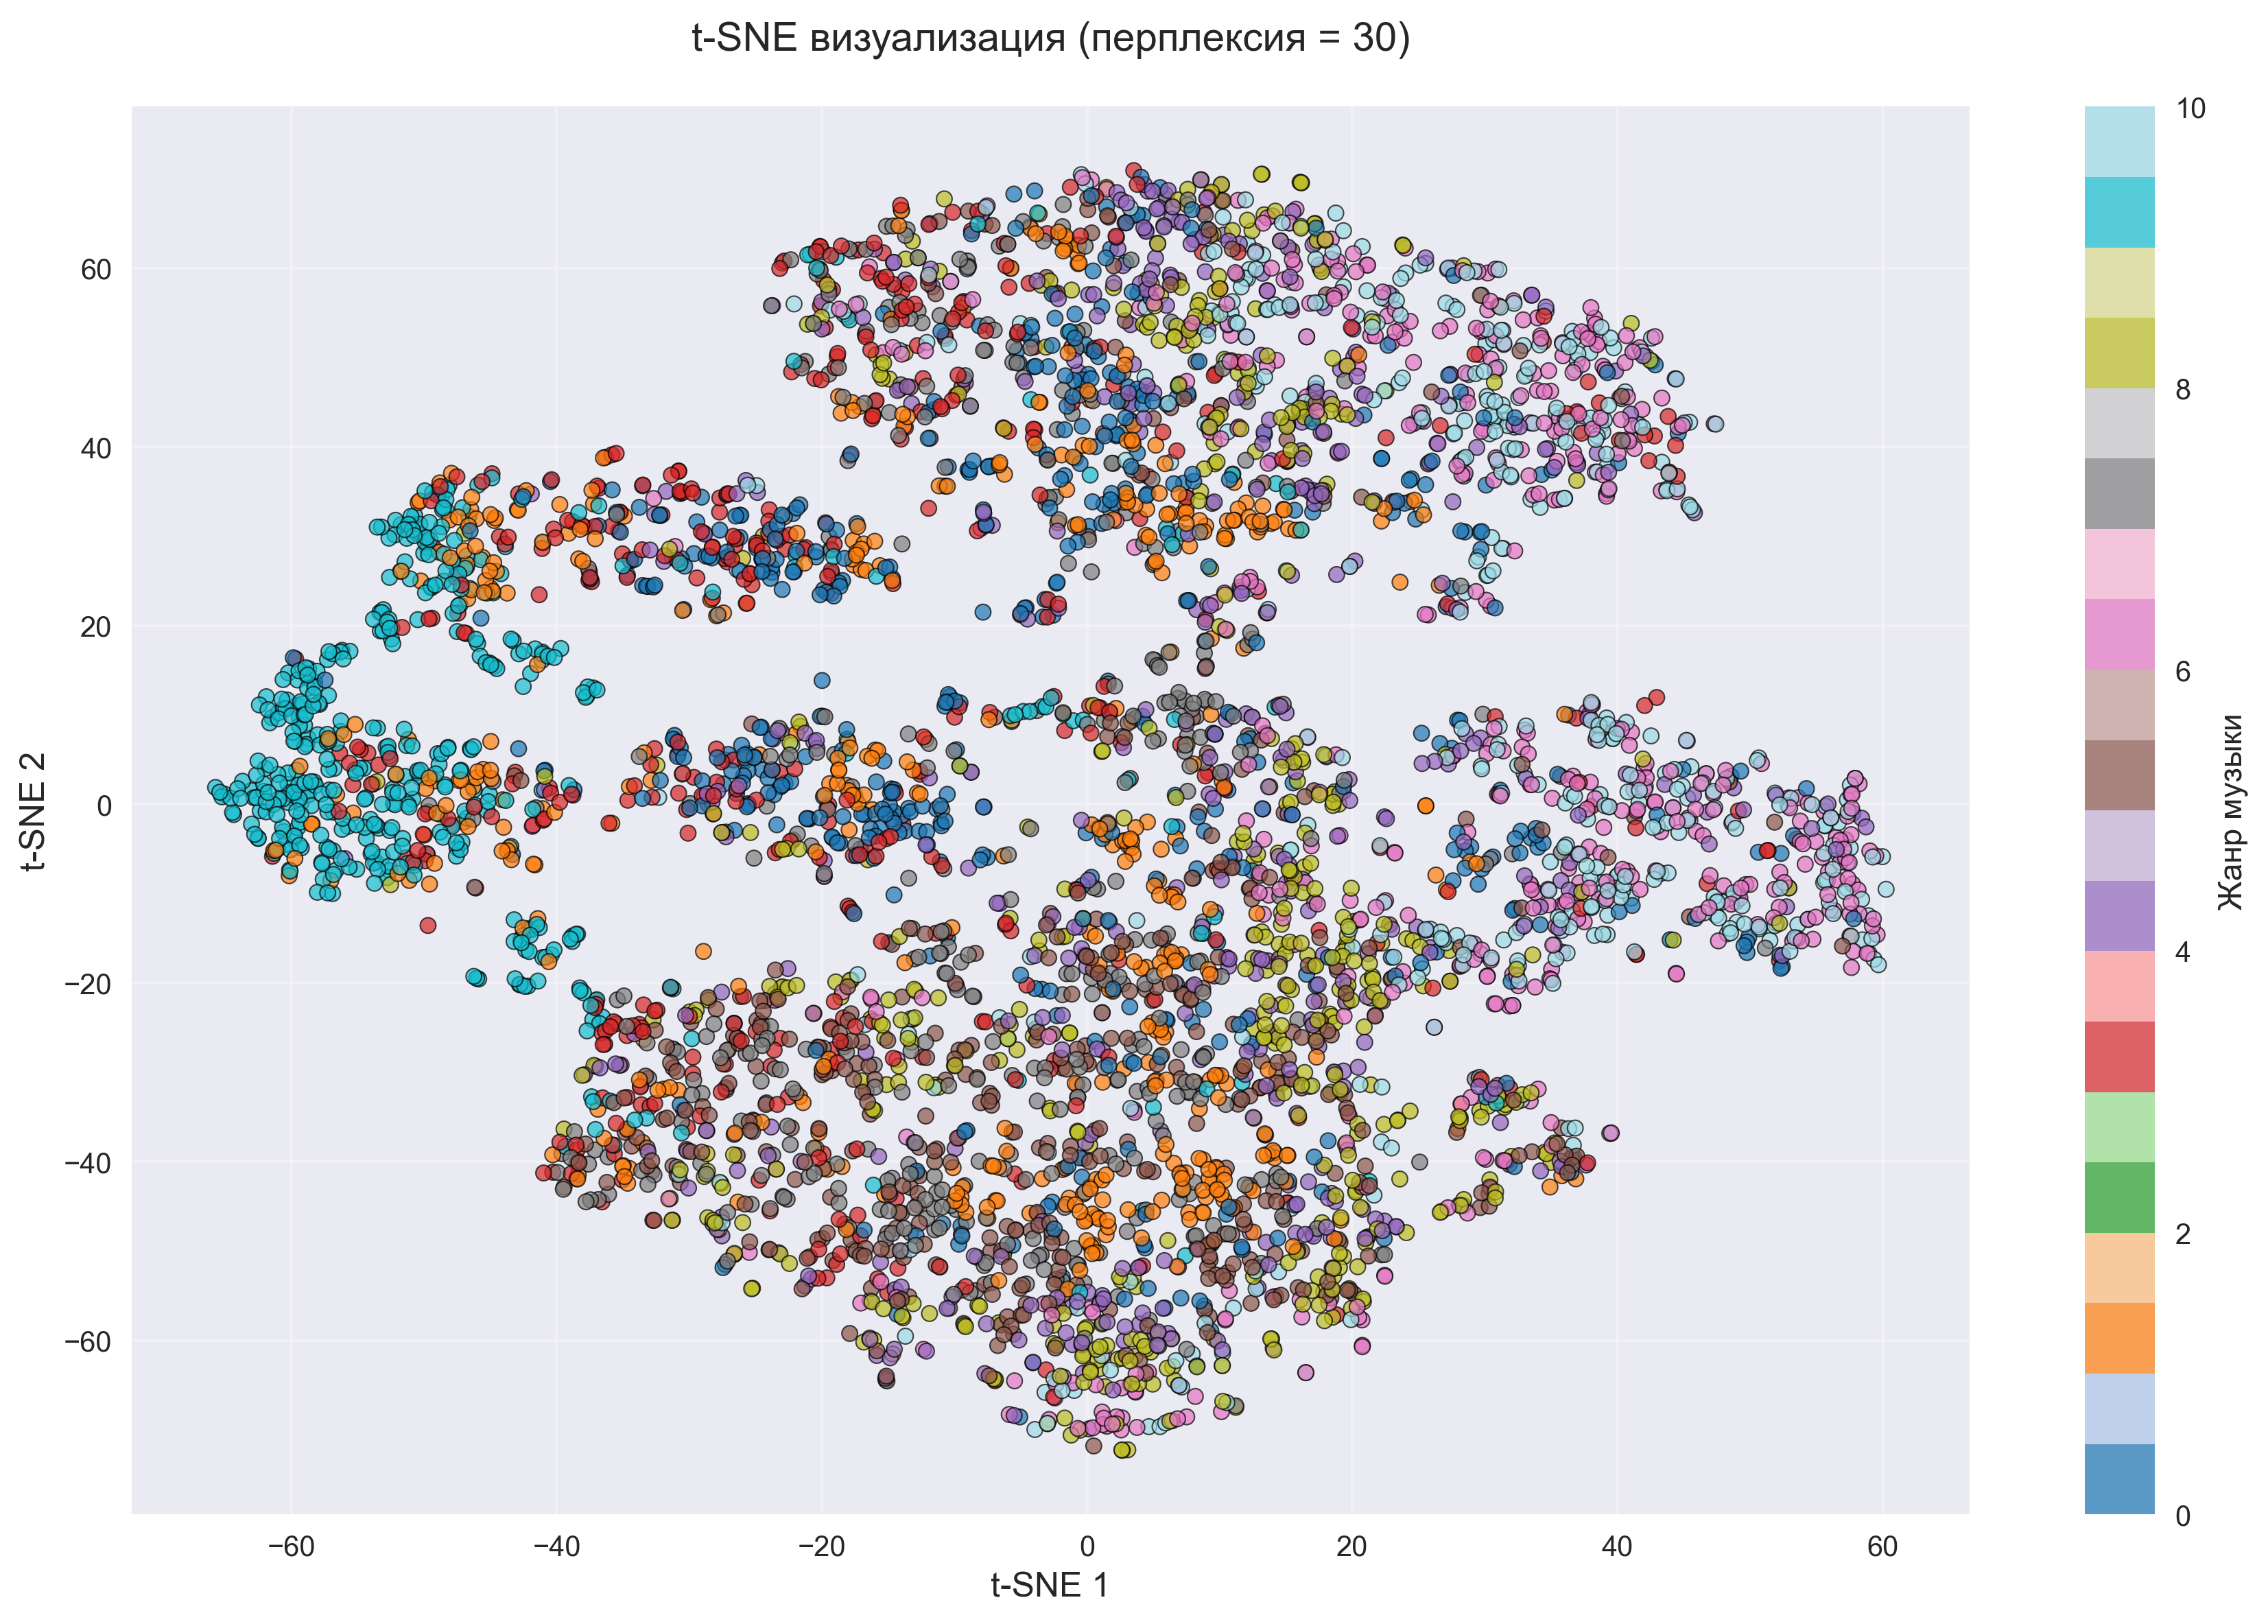
\includegraphics[width=0.9\textwidth]{images/tsne_optimal.png}
    \caption{Оптимальная t-SNE визуализация (перплексия = 30)}
    \label{fig:tsne_optimal}
\end{figure}

Для данного датасета оптимальной оказалась перплексия 30, которая обеспечивает хороший баланс между локальной и глобальной структурой данных.

\section{Анализ влияния параметра перплексии на результат}

\textbf{Влияние перплексии:}

\begin{enumerate}
    \item \textbf{На размер кластеров}: Низкая перплексия создает больше мелких кластеров, высокая -- меньше крупных
    \item \textbf{На разделимость жанров}: Оптимальная перплексия (обычно 30--50) лучше всего разделяет различные жанры
    \item \textbf{На вычислительное время}: Более высокая перплексия требует больше времени на вычисления
    \item \textbf{На стабильность}: Результаты t-SNE могут варьироваться при разных запусках, особенно при низкой перплексии
\end{enumerate}

\textbf{Рекомендации по выбору перплексии:}
\begin{itemize}
    \item Для небольших датасетов ($< 1000$ точек): перплексия 5--15
    \item Для средних датасетов (1000--10000 точек): перплексия 30--50
    \item Для больших датасетов ($> 10000$ точек): перплексия 50--100
\end{itemize}

% Глава 4
\chapter{Сравнительный анализ PCA и t-SNE}

\section{Преимущества и недостатки каждого метода}

\subsection{PCA (Principal Component Analysis)}

\textbf{Преимущества:}
\begin{enumerate}
    \item \textbf{Быстрота вычислений} -- PCA работает очень быстро даже на больших датасетах
    \item \textbf{Детерминированность} -- результаты воспроизводимы и не зависят от случайных начальных условий
    \item \textbf{Интерпретируемость} -- главные компоненты имеют четкую математическую интерпретацию
    \item \textbf{Линейность} -- сохраняет глобальную структуру данных
    \item \textbf{Масштабируемость} -- эффективен для данных любого размера
    \item \textbf{Обратимость} -- можно восстановить исходные данные (с потерей информации)
    \item \textbf{Объясненная дисперсия} -- четкая метрика качества снижения размерности
\end{enumerate}

\textbf{Недостатки:}
\begin{enumerate}
    \item \textbf{Линейность} -- не может уловить нелинейные зависимости в данных
    \item \textbf{Глобальная структура} -- фокусируется на глобальной дисперсии, может терять локальные паттерны
    \item \textbf{Ограниченная визуализация} -- для сложных нелинейных данных может давать менее информативные визуализации
    \item \textbf{Предположения} -- предполагает, что главные направления вариации линейны
\end{enumerate}

\subsection{t-SNE (t-distributed Stochastic Neighbor Embedding)}

\textbf{Преимущества:}
\begin{enumerate}
    \item \textbf{Нелинейность} -- может уловить сложные нелинейные зависимости
    \item \textbf{Локальная структура} -- отлично сохраняет локальные кластеры и близость точек
    \item \textbf{Визуализация} -- создает более информативные и красивые визуализации для сложных данных
    \item \textbf{Кластеризация} -- лучше разделяет различные группы данных
    \item \textbf{Гибкость} -- настраиваемый параметр перплексии позволяет адаптировать метод к данным
\end{enumerate}

\textbf{Недостатки:}
\begin{enumerate}
    \item \textbf{Медленность} -- вычислительно дорогой метод, особенно для больших датасетов
    \item \textbf{Стохастичность} -- результаты могут варьироваться при разных запусках
    \item \textbf{Параметризация} -- требует подбора параметра перплексии
    \item \textbf{Необратимость} -- нельзя восстановить исходные данные
    \item \textbf{Глобальная структура} -- может искажать глобальные расстояния между далекими кластерами
    \item \textbf{Масштабирование} -- сложно применять к новым данным без переобучения
\end{enumerate}

\section{Сравнение результатов на исследуемых данных}

\begin{figure}[H]
    \centering
    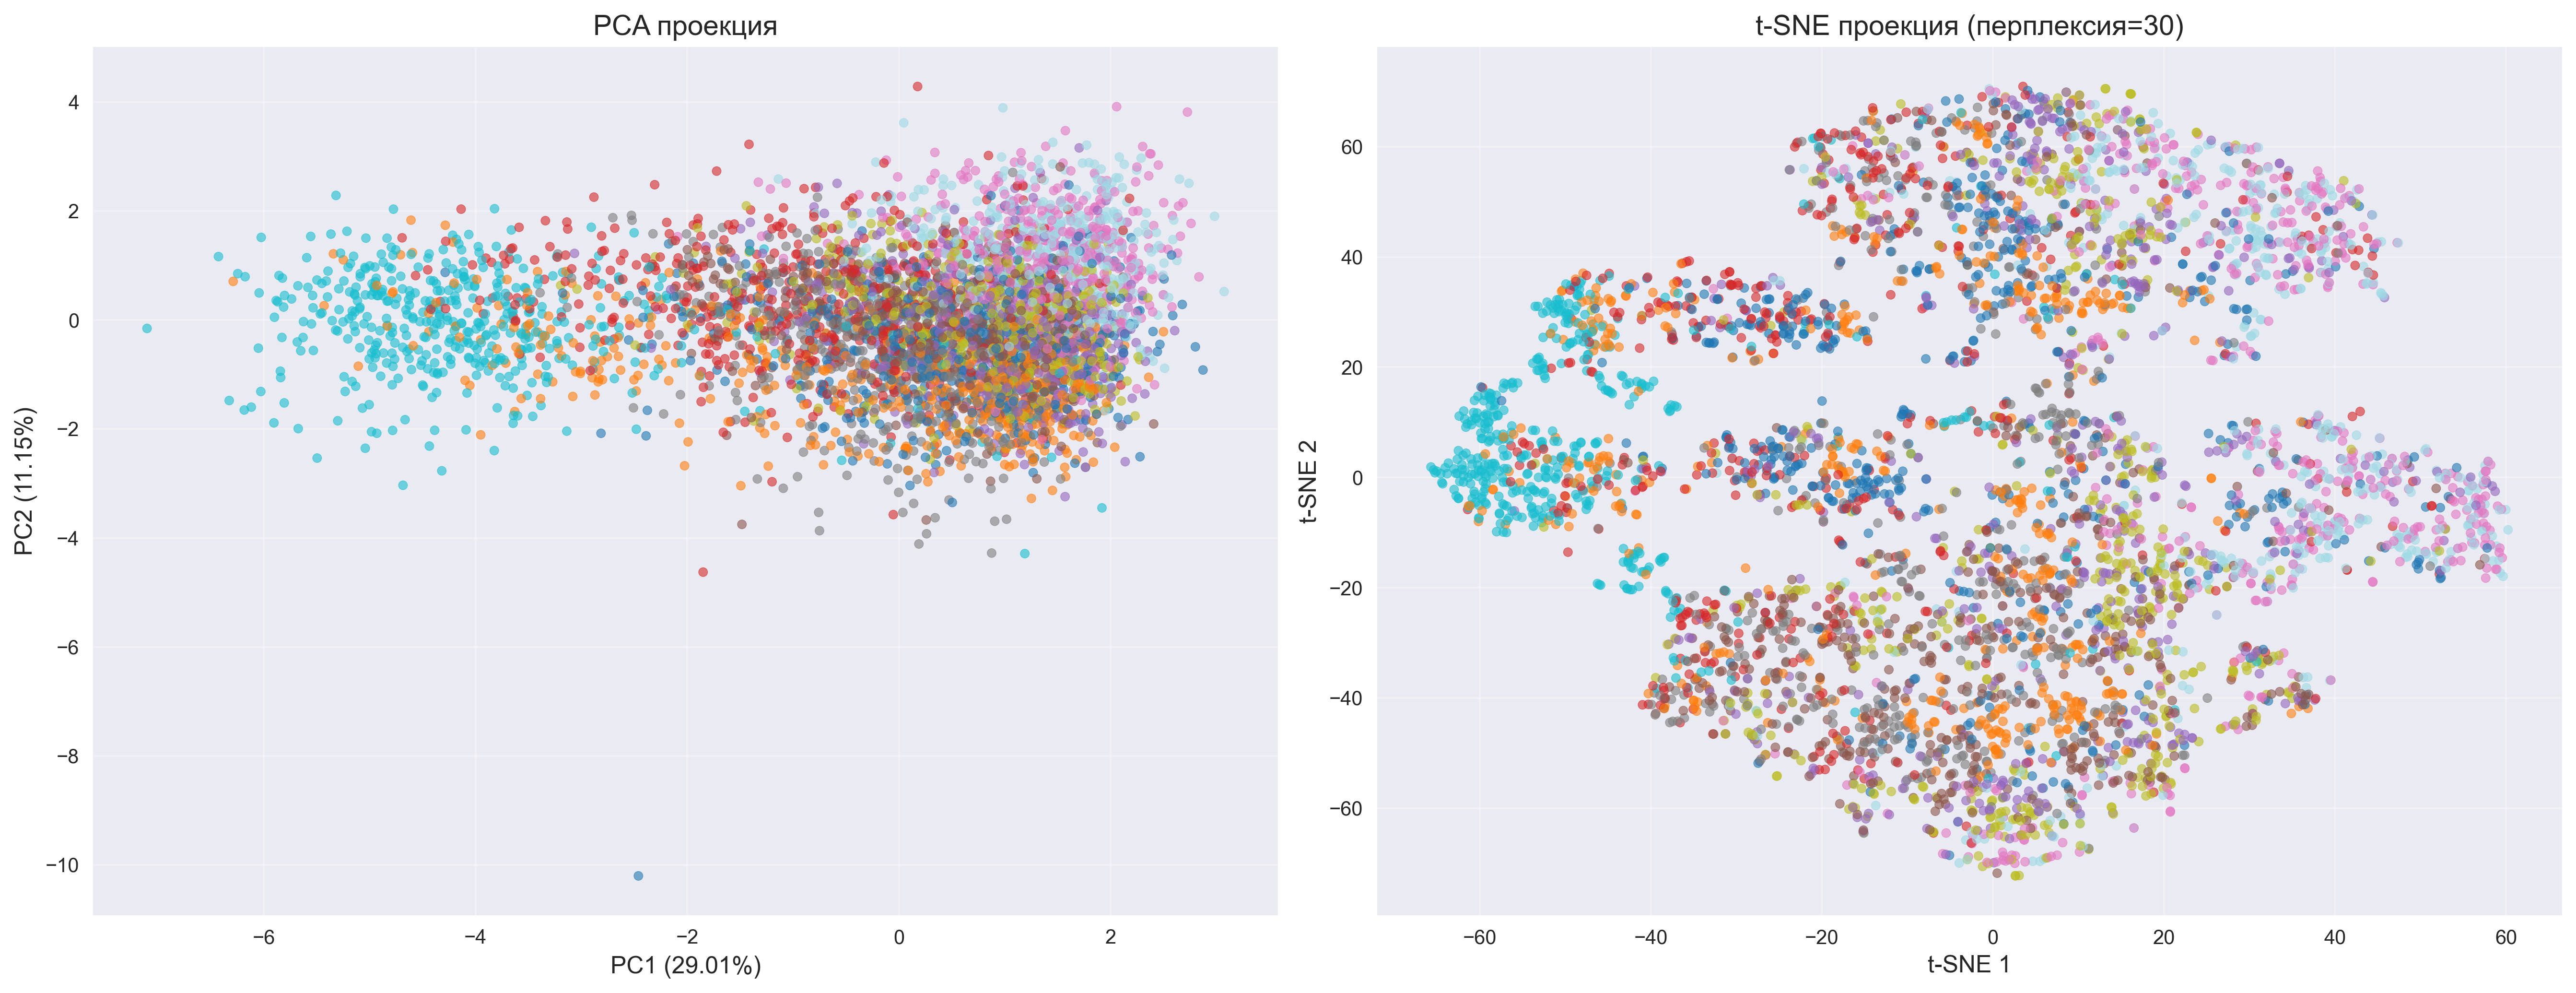
\includegraphics[width=0.95\textwidth]{images/pca_vs_tsne.png}
    \caption{Сравнение PCA и t-SNE}
    \label{fig:comparison}
\end{figure}

\textbf{На данных о музыкальных жанрах:}

\textbf{PCA результаты:}
\begin{itemize}
    \item Хорошо выявляет основные направления вариации в аудио-характеристиках
    \item Позволяет интерпретировать, какие характеристики наиболее важны
    \item Может показывать общие тенденции, но жанры могут перекрываться в проекции
    \item Эффективен для понимания структуры данных в целом
\end{itemize}

\textbf{t-SNE результаты:}
\begin{itemize}
    \item Лучше разделяет различные жанры музыки на отдельные кластеры
    \item Создает более четкую визуализацию различий между жанрами
    \item Показывает локальные сходства между похожими треками
    \item Может выявить скрытые подгруппы внутри жанров
\end{itemize}

\textbf{Ключевые различия:}
\begin{itemize}
    \item PCA показывает глобальную структуру и основные направления вариации
    \item t-SNE показывает локальную структуру и кластеризацию
    \item Для данных о музыке t-SNE часто дает более информативную визуализацию для разделения жанров
    \item PCA лучше подходит для понимания того, какие характеристики важны
\end{itemize}

\section{Рекомендации по использованию методов для различных типов задач}

\subsection{Когда использовать PCA:}

\begin{enumerate}
    \item \textbf{Исследовательский анализ данных (EDA)}
    \begin{itemize}
        \item Быстрое понимание структуры данных
        \item Выявление основных направлений вариации
        \item Определение важных переменных
    \end{itemize}
    
    \item \textbf{Предобработка для машинного обучения}
    \begin{itemize}
        \item Уменьшение размерности перед обучением моделей
        \item Удаление мультиколлинеарности
        \item Ускорение обучения алгоритмов
    \end{itemize}
    
    \item \textbf{Большие датасеты}
    \begin{itemize}
        \item Когда важна скорость вычислений
        \item Когда нужна воспроизводимость результатов
    \end{itemize}
    
    \item \textbf{Интерпретируемость важна}
    \begin{itemize}
        \item Когда нужно понять, какие переменные важны
        \item Когда нужна математическая интерпретация результатов
    \end{itemize}
    
    \item \textbf{Линейные зависимости}
    \begin{itemize}
        \item Когда данные имеют линейную структуру
        \item Когда главные направления вариации линейны
    \end{itemize}
\end{enumerate}

\subsection{Когда использовать t-SNE:}

\begin{enumerate}
    \item \textbf{Визуализация сложных данных}
    \begin{itemize}
        \item Высокоразмерные данные с нелинейной структурой
        \item Данные с множеством кластеров
        \item Когда нужна красивая и информативная визуализация
    \end{itemize}
    
    \item \textbf{Кластеризация и разделение групп}
    \begin{itemize}
        \item Когда важно визуально разделить различные классы
        \item Поиск скрытых кластеров в данных
        \item Анализ сходства между объектами
    \end{itemize}
    
    \item \textbf{Небольшие и средние датасеты}
    \begin{itemize}
        \item Когда вычислительные ресурсы позволяют
        \item Когда важнее качество визуализации, чем скорость
    \end{itemize}
    
    \item \textbf{Нелинейные зависимости}
    \begin{itemize}
        \item Когда данные имеют сложную нелинейную структуру
        \item Когда локальная структура важнее глобальной
    \end{itemize}
    
    \item \textbf{Презентация результатов}
    \begin{itemize}
        \item Для визуализации в отчетах и презентациях
        \item Когда нужно показать кластеризацию данных
    \end{itemize}
\end{enumerate}

\subsection{Комбинированное использование:}

Часто эффективно использовать оба метода:
\begin{enumerate}
    \item \textbf{PCA $\to$ t-SNE}: Сначала применить PCA для уменьшения размерности до 50--100 компонент, затем t-SNE для финальной визуализации
    \item \textbf{PCA для анализа, t-SNE для визуализации}: Использовать PCA для понимания структуры, а t-SNE для презентации результатов
\end{enumerate}

% Выводы
\chapter{Выводы по работе}

\begin{enumerate}
    \item \textbf{Предобработка данных} является критически важным этапом для успешного применения методов уменьшения размерности. Правильная обработка категориальных переменных, удаление неинформативных признаков и стандартизация данных значительно улучшают качество результатов.
    
    \item \textbf{PCA} показал себя как эффективный метод для:
    \begin{itemize}
        \item Быстрого анализа структуры данных
        \item Выявления основных направлений вариации
        \item Интерпретации важности различных характеристик
        \item Работы с большими объемами данных
    \end{itemize}
    
    \item \textbf{t-SNE} продемонстрировал превосходство в:
    \begin{itemize}
        \item Визуализации сложных нелинейных структур
        \item Разделении различных классов (жанров музыки)
        \item Сохранении локальной структуры данных
        \item Создании информативных визуализаций
    \end{itemize}
    
    \item \textbf{Сравнительный анализ} показал, что выбор метода зависит от конкретной задачи:
    \begin{itemize}
        \item Для понимания структуры и интерпретации -- PCA
        \item Для визуализации и кластеризации -- t-SNE
        \item Для комплексного анализа -- комбинация обоих методов
    \end{itemize}
    
    \item \textbf{Параметры методов} (количество компонент для PCA, перплексия для t-SNE) требуют тщательного подбора в зависимости от характеристик данных и целей анализа.
    
    \item \textbf{Практическое применение}: Оба метода нашли широкое применение в анализе данных, машинном обучении и визуализации, и их понимание является важным навыком для специалиста по анализу данных.
\end{enumerate}

% Заключение
\chapter{Заключение}

В ходе лабораторной работы были успешно освоены методы уменьшения размерности данных PCA и t-SNE. Проведен полный цикл анализа: от предобработки данных до сравнительного анализа методов. Полученные результаты демонстрируют различные подходы к решению задачи уменьшения размерности и их применимость в зависимости от конкретных целей исследования.

Работа показала важность правильного выбора метода и его параметров для получения информативных и интерпретируемых результатов анализа данных.

\end{document}

